\documentclass{article}[11pt]
\usepackage[frenchb,english]{babel}
\usepackage[T1]{fontenc}
\usepackage[utf8]{inputenc}
\usepackage{amsmath,amssymb,latexsym}
\usepackage{times}
\usepackage{float}
\usepackage[left=2cm,right=2cm,top=2cm,bottom=2cm]{geometry}
\frenchbsetup{StandardLists=true} % � inclure si on utilise \usepackage[french]{babel}
\usepackage{enumitem}
\usepackage{fancyhdr}
\usepackage{mathrsfs}
\usepackage{graphicx}
%\usepackage[Algorithme]{algorithm}
%\usepackage{algorithmic}
\usepackage{tikz}
\usepackage{tabularx}
\usetikzlibrary{shapes}
\pagestyle{fancy}
\newcommand{\tr}[1]{{\vphantom{#1}}^{\mathit t}{#1}} 
\renewcommand\headrulewidth{1pt}
\fancyhead[L]{Cours 1�re S}
\fancyhead[R]{Yoann Pietri}
\newcounter{theoremecounter}[subsection]
\usepackage{titlesec}
\setcounter{secnumdepth}{3}% enl�ve la num�rotation apr�s les sections
%\renewcommand\thechapter {\Roman{chapter}}

 \setlength{\parindent}{0pt}

\newcommand{\R}{\mathbb{R}}
\newcommand{\N}{\mathbb{N}}
\newcommand{\Q}{\mathbb{Q}}
\newcommand{\Z}{\mathbb{Z}}
\newcommand{\C}{\mathbb{C}}
\newcommand{\K}{\mathbb{K}}
\newcommand{\eqi}{\Leftrightarrow}
\titleformat{\subsubsection}
   {\normalfont\fontsize{11pt}{13pt}\selectfont\bfseries}% apparence commune au titre et au num�ro
   {\thesubsubsection}% apparence du num�ro
   {1em}% espacement num�ro/texte
   {}% apparence du titre

\tikzstyle{theobox} = [draw=black, very thick,
    rectangle, rounded corners, inner sep=10pt, inner ysep=20pt]
\tikzstyle{theotitle} =[fill=white, text=black,rounded corners,draw=black,very thick]

\fancyhead[L]{Contrôle chapitre 5 et 6}

\usepackage{tcolorbox}
\usepackage[c]{esvect}
\newcommand{\covec}[2]{\begin{pmatrix}#1 \\#2 \end{pmatrix}}


\begin{document}
\center
\Large
Contrôle de cours (correction)
\flushleft
\center
Géométrie plane et trigonométrie
\flushleft \normalsize
\subsection*{Exercice 1 (R.O.C., temps conseillé : 10 min) : }
Soient $\vv{u}$ et $\vv{v}$ deux vecteurs 
On suppose $\vv{u} \neq \vv{0}$ et $\vv{v} \neq \vv{0}$ (dans ces cas là, la preuve est immédiate)\newline

Supposons $\vv{u}$ et $\vv{v}$ colinéaires. Alors, il existe $k\in \R^*$ tel que $$\vv{u} = k\vv{v}$$
Alors 
$$x = kx'$$
$$y = ky'$$
Alors $$xy' - x'y = kx'y' - x'ky' = 0$$

Réciproquement, supposons que $$xy'-x'y = 0$$
$\vv{u} \neq \vv{0}$ donc au moins une de ses coordonnées est non nulle. On suppose $x \neq 0$ (la démonstration est la même si c'est $y\neq 0$)\newline

Alors $$y' = \frac{x'}{x}y$$
On pose alors $k = \frac{x'}{x}$ 
$$kx = k\frac{x'}{x} = x'$$
$$ky = \frac{x'}{x} y = y'$$
donc 
$$\vv{v} = k\vv{u}$$ 
donc les vecteurs sont colinéaires

\subsection*{Exercice 2 (temps conseillé : 20 min) : }
\begin{enumerate}
\item On a (lecture graphique) 
$$\boxed{A(3,5;1)}$$
$$\boxed{B(2,5;3)}$$
$$\boxed{C(-1,5;2)}$$
\item On a $$I\left(\frac{x_A + x_B}{2}; \frac{y_A+y_B}{2}\right)$$
$$I\left(\frac{3,5 + 2,5}{2},\frac{1+3}{2}\right)$$
$$\boxed{I(3,2)}$$
\item On a $$\vv{AB} \covec{x_B-x_A}{y_B - y_A} = \covec{2,5-3,5}{3-1}$$
$$\boxed{\vv{AB} \covec{-1}{2}}$$
\item On considère deux points $A_1$ et $A_2$ de $\mathscr{D}$, on prend par exemple $$A_1 (0;2)$$ et $$A_2(3,0)$$ et calcule $\vv{A_1A_2}$ : $$\vv{A_1A_2} \covec{0-3}{2-0}$$ ainsi $$\boxed{\covec{-3}{2} \text{ est un vecteur directeur de } \mathscr{D}}$$
\item On utilise le vecteur directeur calculé à la question précédente et on utilise le fait que $A_1 (0;2)$ soit un point de $\mathscr{D}$ 
$$\mathscr{D} : 2x + 3y = 2\times 0 + 3\times 2$$
$$\boxed{\mathscr{D} : 2x + 3y = 6}$$
ou sous la forme d'une équation réduite
$$\boxed{\mathscr{D} : y = -\frac{2}{3}x+2}$$
\item Si $D(x_D,y_D)$ est tel que $ABCD$ soit un parallélogramme alors $$\vv{AB} = \vv{DC}$$
$$\covec{-1}{2} = \covec{-1,5 -x_D}{2-y_D}$$
$$\left\{\begin{array}{l} -1,5 -x_D = -1\\ 2-y_D = 2\end{array}\right.$$
$$\left\{\begin{array}{l} x_D = -0,5\\ y_D = 0\end{array}\right.$$
Finalement 
$$\boxed{D(-0,5;0)}$$
\end{enumerate}
\subsection*{Exercice 3 (Coordonnées polaires, temps conseillé : 25 min) : }
\begin{enumerate}
\item Soit $\vv{u_1}$ et $\vv{u_2}$ deux vecteurs non colinéaires. Soit $\vv{v}$ un vecteur du plan. Alors il existe un unique couple de réels $(\lambda,\mu)$ tel que $$\vv{v} = \lambda \vv{u_1} + \mu \vv{u_2}$$
\item On a $$\cos(\theta) \times \cos(\theta) - \sin(\theta)\times (-\sin(\theta)) = \cos(\theta)^2 + \sin(\theta)^2 = 1 \neq 0$$
\item Bah oui...
\item On a $$\covec{x}{y} = \lambda \covec{\cos(\theta)}{\sin(\theta)} + \mu \covec{-\sin(\theta)}{\cos(\theta)}$$
$$\covec{x}{y} =  \covec{\lambda\cos(\theta)}{\lambda\sin(\theta)} +  \covec{-\mu\sin(\theta)}{\mu\cos(\theta)}$$
$$\covec{x}{y} =  \covec{\lambda\cos(\theta)-\mu\sin(\theta)}{\lambda\sin(\theta) +\mu\cos(\theta)}$$
$$\left\{\begin{array}{l l l l l} x & = & \lambda \cos(\theta) & - & \mu \sin(\theta) \quad (1) \\ y & = & \lambda \sin(\theta) & + &\mu \cos(\theta) \quad (2)\end{array}\right.$$
\item 
$$\cos(\theta) \times (1) + \sin(\theta) \times (2)$$
$$x\cos(\theta) + y \sin(\theta) = \lambda\cos(\theta)^2 -\mu\cos(\theta)\sin(\theta) + \lambda \sin(\theta)^2 + \mu\cos(\theta)\sin(\theta)$$
$$x\cos(\theta) + y \sin(\theta) = \lambda(\cos(\theta)^2 + \sin(\theta)^2)$$
$$\boxed{x\cos(\theta) + y \sin(\theta) = \lambda}$$
$$-\sin(\theta) \times (1) + \cos(\theta) \times (2)$$
$$-\sin(\theta)x + \cos(\theta)y = -\lambda \sin(\theta)\cos(\theta) + \mu \sin(\theta)^2 + \lambda \sin(\theta) \cos(\theta) + \mu \cos(\theta)^2$$
$$-\sin(\theta)x + \cos(\theta)y = \mu(\sin(\theta)^2 + \cos(\theta)^2)$$
$$\boxed{-\sin(\theta)x + \cos(\theta)y = \mu}$$
\item Correspond à une rotation de $\frac{\pi}{4}$ pour les vecteurs de la base canonique :\newline
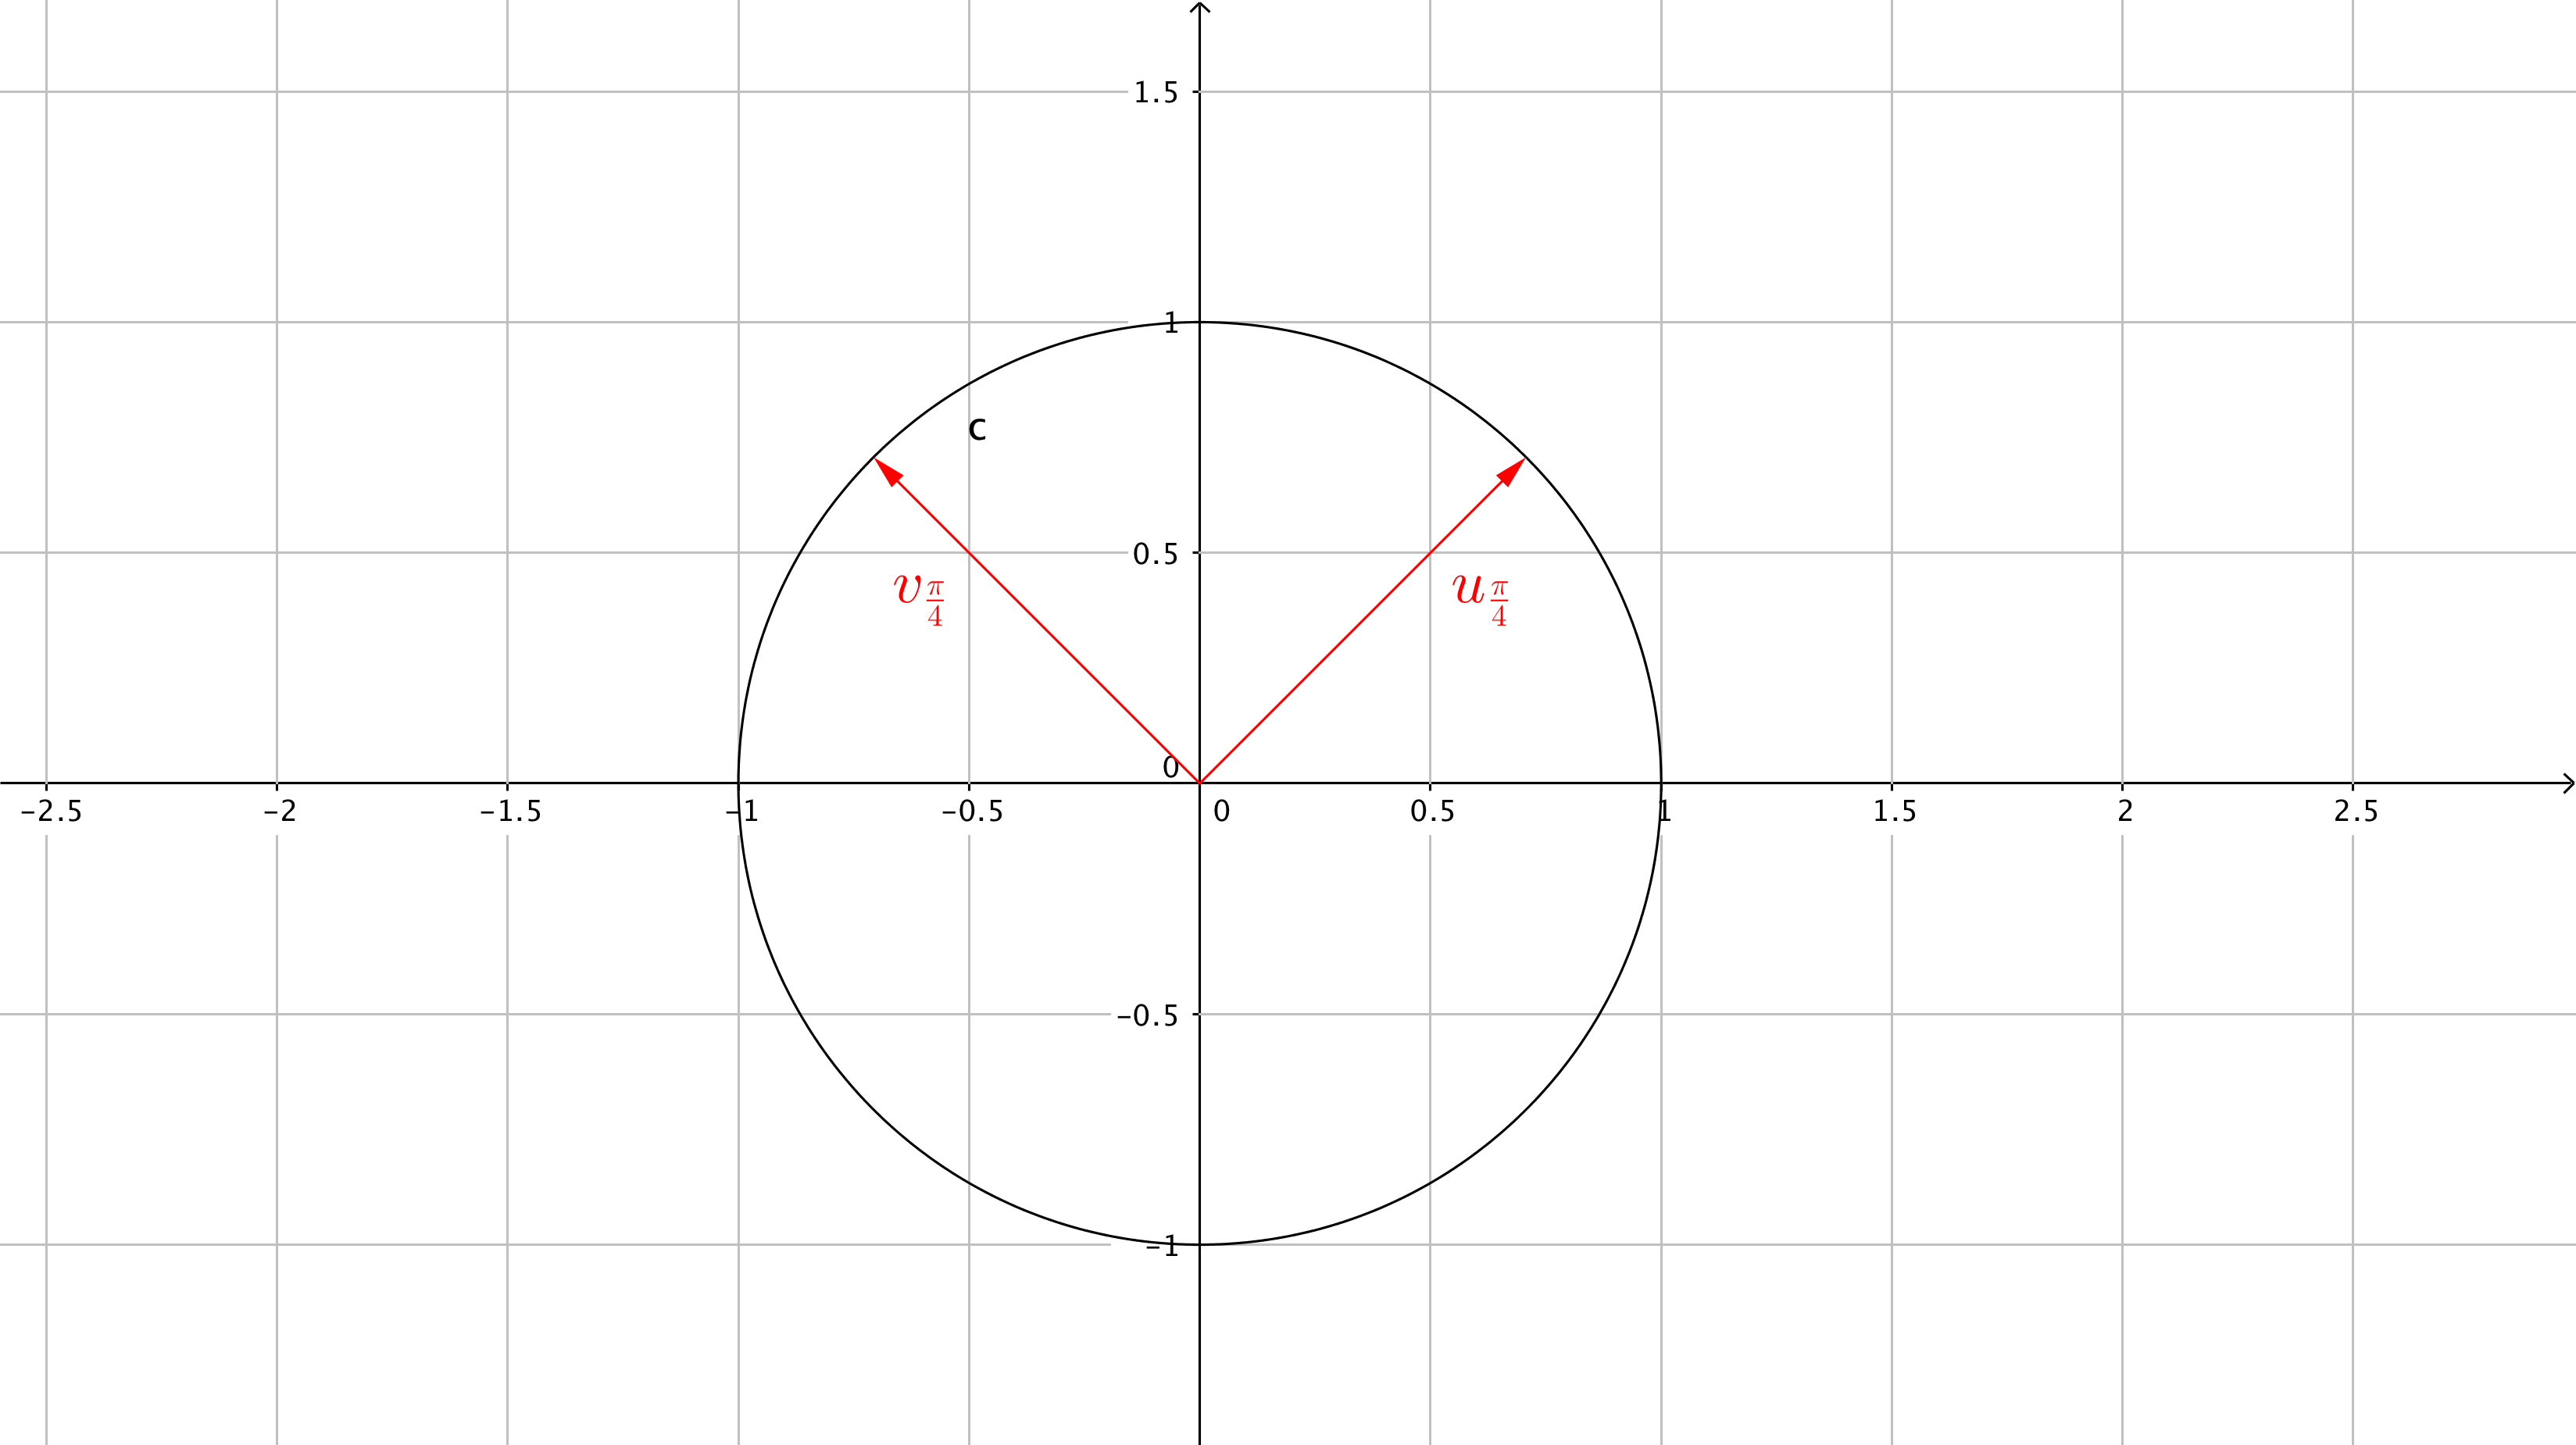
\includegraphics[scale=0.2]{chap5_corr_ill1.png}
\item On calcule $\lambda$ et $\mu$ pour $\displaystyle \covec{\frac{1}{2}}{1}$ grâce à la question 5 : 
$$\lambda = \frac{1}{2}\cos(\frac{\pi}{4}) + 1 \times \sin(\frac{\pi}{4})$$
$$\lambda = \frac{\sqrt{2}}{4} + \frac{\sqrt{2}}{2}$$
$$\boxed{\lambda = \frac{3\sqrt{2}}{4}}$$
$$\mu = 1\times \cos(\frac{\pi}{4}) - \frac{1}{2}\sin(\frac{\pi}{4})$$
$$\mu = \frac{\sqrt{2}}{2} - \frac{\sqrt{2}}{4}$$
$$\boxed{\mu = \frac{\sqrt{2}}{4}}$$
Ainsi $$\boxed{\covec{\frac{1}{2}}{1} = \frac{3\sqrt{2}}{4}u_{\frac{\pi}{4}} + \frac{\sqrt{2}}{4}v_{\frac{\pi}{4}}}$$
\item Le cas $\theta =0$ correspond au cas que l'on utilise quasiment tout le temps, c'est à dire une décomposition selon $\covec{1}{0}$ et $\covec{0}{1}$
\end{enumerate}
$$\star \star \star$$
\center
FIN DU SUJET
\end{document}